\documentclass[twoside]{article}

\usepackage{amsmath,amsthm,amssymb,graphicx}
\usepackage{hyperref}
\usepackage[numbers]{natbib}
\usepackage{float}
\usepackage{bbm}

\theoremstyle{definition}
\newtheorem{thm}{Theorem}[section]
\newtheorem{lem}[thm]{Lemma}
\newtheorem{prop}[thm]{Proposition}
\newtheorem{cor}[thm]{Corollary}
\newenvironment{pf}{{\noindent\sc Proof. }}{\qed}
\newenvironment{map}{\[\begin{array}{cccc}} {\end{array}\]}

\newcommand{\comment}[1]{}
\theoremstyle{definition}
\newtheorem*{defn}{Definition}
\newtheorem*{exmp}{Example}
\newtheorem*{prob}{Problem}

\theoremstyle{remark}
\newtheorem*{rem}{Remark}
\newtheorem*{note}{Note}
\newtheorem*{exer}{Exercise}

\setlength{\oddsidemargin}{0.25 in}
\setlength{\evensidemargin}{-0.25 in}
\setlength{\topmargin}{-0.6 in}
\setlength{\textwidth}{6.5 in}
\setlength{\textheight}{8.5 in}
\setlength{\headsep}{0.75 in}
\setlength{\parindent}{0 in}
\setlength{\parskip}{0.1 in}

\newcommand{\widgraph}[2]{\includegraphics[keepaspectratio,width=#1]{#2}}
\newcommand{\widgraphr}[3]{\includegraphics[keepaspectratio,width=#1,angle=#3]{#2}}

\newcommand{\lecture}[4]{
   \pagestyle{myheadings}
   \thispagestyle{plain}
   \newpage
   \setcounter{page}{1}
   \noindent
   \begin{center}
   \framebox{
      \vbox{\vspace{2mm}
    \hbox to 6.28in { {\bf Stat365/665 (Spring 2015) Data Mining and Machine Learning \hfill Lecture: #4} }
       \vspace{6mm}
       \hbox to 6.28in { {\Large \hfill #1  \hfill} }
       \vspace{6mm}
       \hbox to 6.28in { {\it Lecturer: #2 \hfill Scribe: #3} }
      \vspace{2mm}}
   }
   \end{center}
   \markboth{#1}{#1}
   \vspace*{4mm}
}


%%%%%%%
% Some commonly used notation
%%%%%%%

\def\R{{\mathbb R}}
\def\X{{\mathcal X}}
\def\Y{{\mathcal Y}}
\def\H{{\mathcal H}}
\def\E{{\mathbb E}}
\def\sign{{\rm sign}}

\newcommand{\percent}{$\%$}

\begin{document}

\lecture{Data Mining and Machine Learning}{Sahand Negahban}{Leon Lixing Yu}{16}
\section{Boosting and overfitting}
The decision tree I used is matlab function $fitctree$, that takes inputs, $Y$, $X$, $weights$, and $maxNumSplits$. The maximum number of splits are used to control the depth of the tree.\\
If the $maxNumSplits$ is $3$, the depth of the tree is 2. likewise, if the $maxNumSplits$ is $4$, the depth of the tree is 3. Since we are given the depth of the tree as $3$, I choose the $maxNumSplits = 4$. \\
The code for this problem is attached in $Appendix-A$.The figures below shows the test errors while changing the number of iterations with fixed tree depth.  

\begin{figure}[H]
\centering
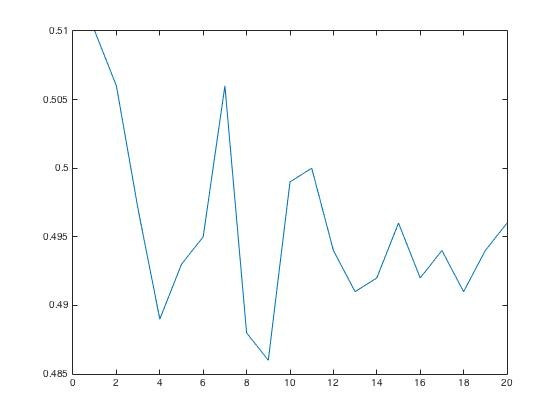
\includegraphics[width=120mm]{problem1_1.jpg}
\caption{test error for upto 20 iterations.I can see a dip at 9th iteration. The testing error and then fluctuates alone the similiar domain.}
\end{figure}

\begin{figure}[H]
\centering
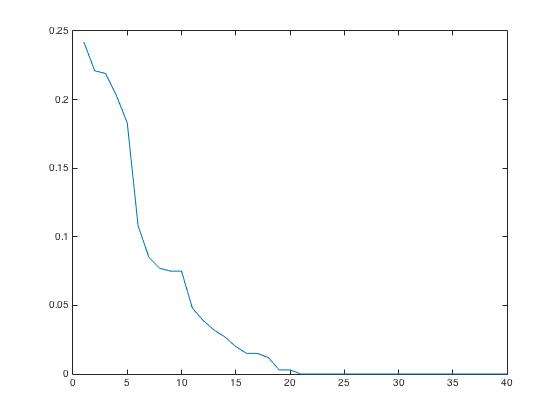
\includegraphics[width=120mm]{problem1_2.jpg}
\caption{training error for upto 40 iterations.I can see at around 20th iteration, the boosting converges to 0 error, meaning everything after 20th iteration is for sure overfitting. Also, since the dip happens at 9th iteration during testing, I claim that the best fit is around 9th iteration, and any work done beyond 9th iteration is considered overfitting. }
\end{figure}

The figure below shows the graph for testing error with incremental tree depth while fixing the iteration number to $3$
\begin{figure}[H]
\centering
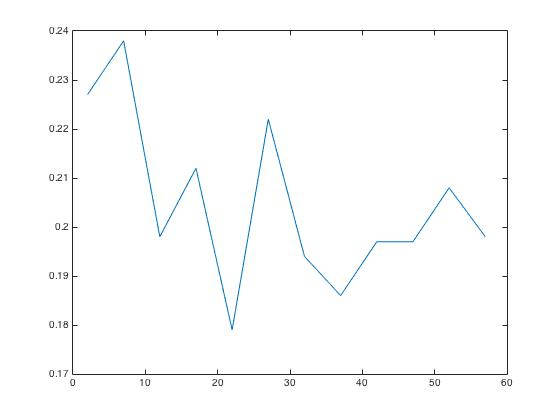
\includegraphics[width=120mm]{problem1_3.jpg}
\caption{training error for upto 40 iterations.I can see at around 20th iteration, the boosting converges to 0 error, meaning everything after 20th iteration is for sure overfitting. Also, since the dip happens at 9th iteration during testing, I claim that the best fit is around 9th iteration, and any work done beyond 9th iteration is considered overfitting. }
\end{figure}







\end{document}
